%!TEX TS-program = xelatex
\documentclass[]{friggeri-cv}
\usepackage{afterpage}
\usepackage{hyperref}
\usepackage{color}
\usepackage{xcolor}
\hypersetup{
    pdftitle={},
    pdfauthor={},
    pdfsubject={},
    pdfkeywords={},
    colorlinks=false,       % no lik border color
   allbordercolors=white    % white border color for all
}
\addbibresource{bibliography.bib}
\RequirePackage{xcolor}
\definecolor{pblue}{HTML}{0395DE}

\begin{document}
\header{Rafsan}{Jani}
      {Electrical Engineer}
      
% Fake text to add separator      
\fcolorbox{white}{gray}{\parbox{\dimexpr\textwidth-2\fboxsep-2\fboxrule}{%
.....
}}

% In the aside, each new line forces a line break
\begin{aside}
  \section{Address}
   Sufia Manjil, 169/2/A, Uttar Kunipara, 
   Shanti Niketon, Tejgaon, Dhaka-1208
    ~
  \section{Tel \& Skype}
    +880 183 1615210
    Rafsan Jani
    ~
  \section{Mail}
    \href{mailto:rafsan.buet.10@gmail.com}{\textbf{rafsan.buet.10@}\\gmail.com}
    \href{mailto:rafsan.buet.10@hotmail.com}{\textbf{rafsan.buet.10@}\\hotmail.com}
    ~
  \section{Web \& Git}
    \href{https://rafsanjanichowdhury.github.io}{rafsan.github.io}
    \href{https://github.com/rafsanjanichowdhury}{github.com/rafsan}
    ~
  \section{Programming}
    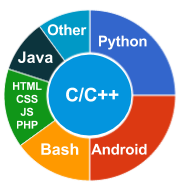
\includegraphics[scale=0.62]{img/programming.png}
    ~
  \section{OS Preference}
    \textbf{GNU/Linux}
\includegraphics[scale=0.40]{img/5stars.png}
    \textbf{Windows}
\includegraphics[scale=0.40]{img/4stars.png}
    \textbf{MacOS}
\includegraphics[scale=0.40]{img/3stars.png}
    \textbf{Solaris}
\includegraphics[scale=0.40]{img/2stars.png}
    ~
  \section{Personal Skills}
    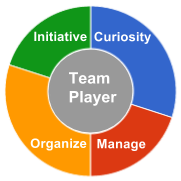
\includegraphics[scale=0.62]{img/personal.png}
    ~
\end{aside}

\section{Experience}
\begin{entrylist}
  \entry
    {10/16 - Now}
    {Quantum Gravity Researcher}
    {Gulshan, Dhaka}
    {Design and development of algorithms of Deep Learning. Integration of Quantum Gravity and Consciousness with Deep Learning\\}
  \entry
    {03/16 - 09/16}
    {UX \& UI Designer}
    {Procyon Inc.}
    {Design and development of Web Applications, Web Solutions, monitoring and Evolution of User Experiences\\}
    \entry
    {01/13 - 03/16}
    {Freelance Developer \& Problem Setter}
    {Bangladesh Math Olympiad}
    {Problem Setting, Test Taking and Test Paper Evaluation\\}
\end{entrylist}

\section{Education}
\begin{entrylist}
  \entry
    {2016 - Now}
    {Studying M.Sc. in Theoretical Physics}
    {University of Dhaka, Bangladesh}
    {Developing the first-principles of Quantum Gravity Theory.\\
    \textbf{Main Concentrations:} Advanced Quantum Mechanics, Relativistic Quantum Field Theory, Statistical Mechanics, Particle Physics, Strong Interactions: Effective Field Theories of QCD.\\}
    \entry
    {2011 - 2016}
    {Bachelor's Degree in EEE}
    {Bangladesh University of Engg. \& Tech., Dhaka}
    {\textbf{Main Concentrations:} Physics and Mathematics, Programming, Power System, Electrical instruments, Telecommunication Systems, Digital and Analogical Electronics.\\
    \emph{\textbf{Title of the Thesis:} "Optimization of Gigabit Ethernet Passive Optical Network Using Advanced Polling and Dynamic Bandwidth Allocation".}\\
    \emph{\textbf{Thesis Supervisor} - Dr. Mohammad Faisal, Associate Professor, EEE, BUET}\\}
  \entry
    {2008 - 2010}
    {Higher Secondary Certificate}
    {Notre Dame College, Dhaka, Bangladesh}
    {\textbf{Group:} Science.\\
    \textbf{Main subjects:} Matematics, Physics, Chemistry and Biology.}
\end{entrylist}

\section{Certifications}
\begin{entrylist}
  \entry
    {Dec 12, 2015}
    {Machine Learning}
    {Coursera. Stanford Online}
    {\emph{machine learning, datamining, and statistical pattern recognition}\\\textbf{Course Instructor:} Andrew Ng., Associate Professor, Stanford University}
 % \entry
 %   {Dec 19, 2016}
 %   {The Arduino Platform and C Programming}
 %   {Coursera. Stanford Online}
 %   {\emph{Building digital devices and interactive objects that can sense and control the physical world around them.}\\\textbf{Course Instructor:}  Ian Harris, Associate Professor, UC, Irvine}
\end{entrylist}

\section{Achievements}
\begin{entrylist}
  \entry
    { }
    {48th Position in Rajshahi Board in SSC Examination}
    { }
    { }
  \entry
    { }
    {Runner Up in National Math Olympiad 2009}
    { }
    { }
  \entry
    { }
    {Champion in National Astronomy and Astrophysics Olympiad 2010}
    { }
    { }
\end{entrylist}

\newpage

\section{Skills}
\begin{entrylist}
  \entry
    { }
    {Circuit designing and CAD}
    {Debugging, synthesizing and analysing electrical circuits.}
    {Very good Knowledge in the software packages like Orcad, P-Spice, Eagle, MATLAB, PSAF to simulate circuits \\}
  \entry
    { }
    {Basic PLC and Microcontrollers}
    {Arduino, AVR and Basic PLC programming}
    {sufficient knowledge of Digital electronics and different programming languages for solving different problems.\\}
  \entry
    { }
    {Repairing, Troubleshooting \& Monitoring}
    { }
    {Repairing machines or systems using the needed tools, Determining causes of operating errors and deciding what to do about it and make sure a machine is working properly.}    
\end{entrylist}

\begin{aside}
~
~
~
  \section{Places Lived}
    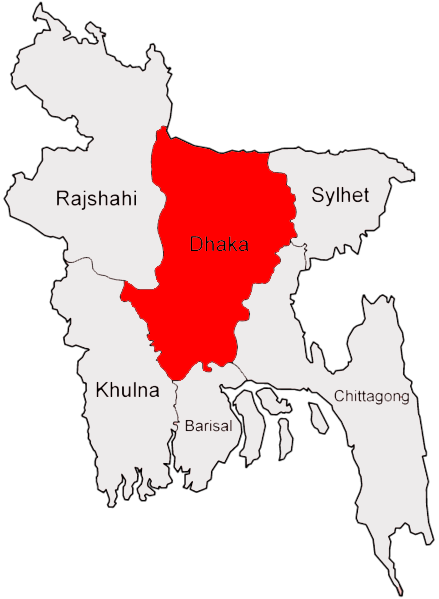
\includegraphics[scale=0.18]{img/italia.png}
    ~
  \section{Languages}
    \textbf{Bangla}
\includegraphics[scale=0.40]{img/5stars.png}
    \textbf{English}
\includegraphics[scale=0.40]{img/4stars.png}
    \textbf{French}
\includegraphics[scale=0.40]{img/2stars.png}
\end{aside}

\section{Notable Projects}
\begin{entrylist}
  \entry
    {Project 1}
    {INTELLIGENT POWER SHARING OF TRANSFORMERS WITH AUTO PROTECTION}
    { }
    { }
  \entry
    {Project 2}
    {DIGITAL OSCILLOSCOPE USING ARDUINO (Micro controller Project)}
    { }
    { }
  \entry
    {Project 3}
    {RUBIC's CUBE SOLVER using MATLAB}
    { }
    { }    
\end{entrylist}

\section{Publications}
H. A. Rafsan, A. H. Chowdhury\\
\textbf{"A Research Paper Published in IJSRT, titling of 'A New Parallelization Strategy for the Solution of the Time-Dependent Three Dimensional Maxwell Equations"}\\
\emph{International Journal of Science Research and Technology (IJSRT 2014), Mumbai, India, July 7-10, 2014}
\\

\section{Referee}

\textbf{Dr. Abdul Hasib Chowdhury (Adviser)}
\begin{innerlist}
\item[] Associate Professor in EEE \\
Department of Electrical \& Electronic Engineering \hfill {\textbf{Phone:} 01711901568}\\
Bangladesh University of Engineering and Technology \hfill{\textbf{E-mail:} hasib@eee.buet.ac.bd}\\
\end{innerlist}

\\
\\

\textbf{Dr. Mohammad Faisal (Thesis Supervisor)}
\begin{innerlist}
\item[] Associate Professor in EEE \\
Department of Electrical \& Electronic Engineering \hfill {\textbf{Phone:} 01926714764}\\
Bangladesh University of Engineering and Technology \hfill{\textbf{E-mail:} mdfaisal@eee.buet.ac.bd}\\
\end{innerlist}


%\begin{flushleft}
%\emph{January 14th, 2014}
%\end{flushleft}
\begin{flushright}
\emph{\\ 
\\
\\ Rafsan Jani}
\end{flushright}

%%% This piece of code has been commented by Karol Kozioł due to biblatex errors. 
% 
%\printbibsection{article}{article in peer-reviewed journal}
%\begin{refsection}
%  \nocite{*}
%  \printbibliography[sorting=chronological, type=inproceedings, title={international peer-reviewed conferences/proceedings}, notkeyword={france}, heading=subbibliography]
%\end{refsection}
%\begin{refsection}
%  \nocite{*}
%  \printbibliography[sorting=chronological, type=inproceedings, title={local peer-reviewed conferences/proceedings}, keyword={france}, heading=subbibliography]
%\end{refsection}
%\printbibsection{misc}{other publications}
%\printbibsection{report}{research reports}


\end{document}
